\section{Particle flow event reconstruction}
\label{sec:reco-pf}

Particle flow (PF) \nomenclature{PF}{Particle flow} 
event reconstruction aims to reconstruct and identify
all stable particles in an event. 
In this context, particles are considered stable if
they have a mean lifetime comparable to that of the charged pion
($\left<\tau\right> = 10^{-8}$~s).
These stable particles include electrons, muons, 
photons, charged hadrons, and neutral hadrons.  
The reconstruction process begins by identifying 
fundamental ``elements'': charged particle tracks
and calorimetric energy clusters, which are then 
topologically linked together into ``blocks.''
The PF algorithm then interprets these 
blocks in terms of particles.
Once obtained, this list of interpreted particles
is used as if it came from an event generator to build
jets and to calculate a \met~measurement.
A visualisation of the PF treatment of a hadronic jet
with four constituent particles ($\pi^+$, $\pi^-$, $\pi^0$, $\text{K}_{\text{L}}^0$)
and a \pt~of 65 GeV is shown in Figure \ref{fig:pf} \cite{pf-1}.

\begin{figure}
  \centering
  \begin{subfigure}[b]{0.55\textwidth}
    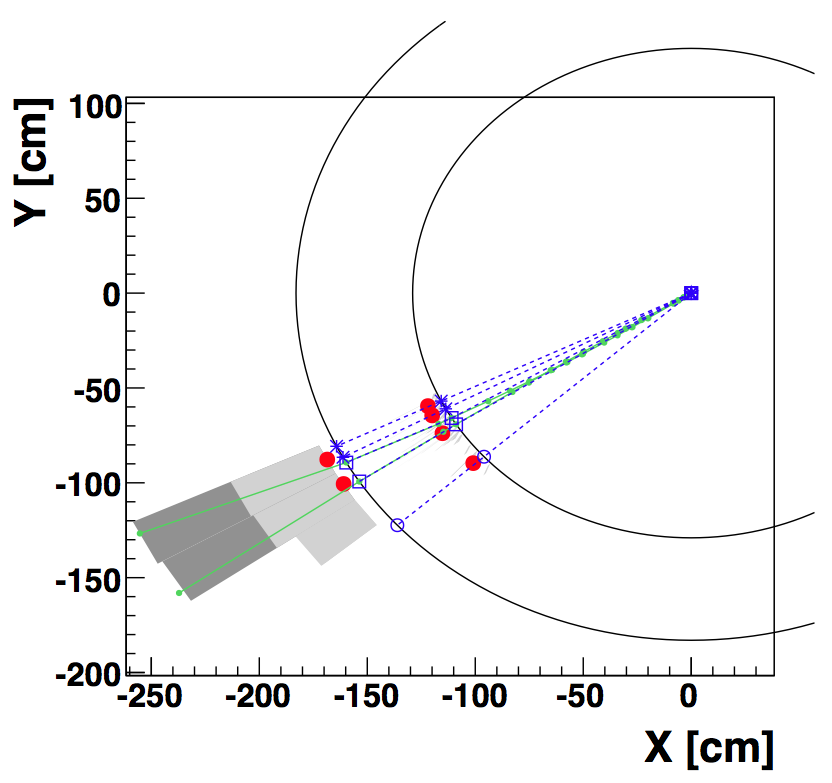
\includegraphics[width=\textwidth]{tex/reco/fig/reco-pf-1.png}
    \caption{$r-\phi$ plane}
    \label{fig:pf-1}
  \end{subfigure} \\
  \begin{subfigure}[b]{0.44\textwidth}
    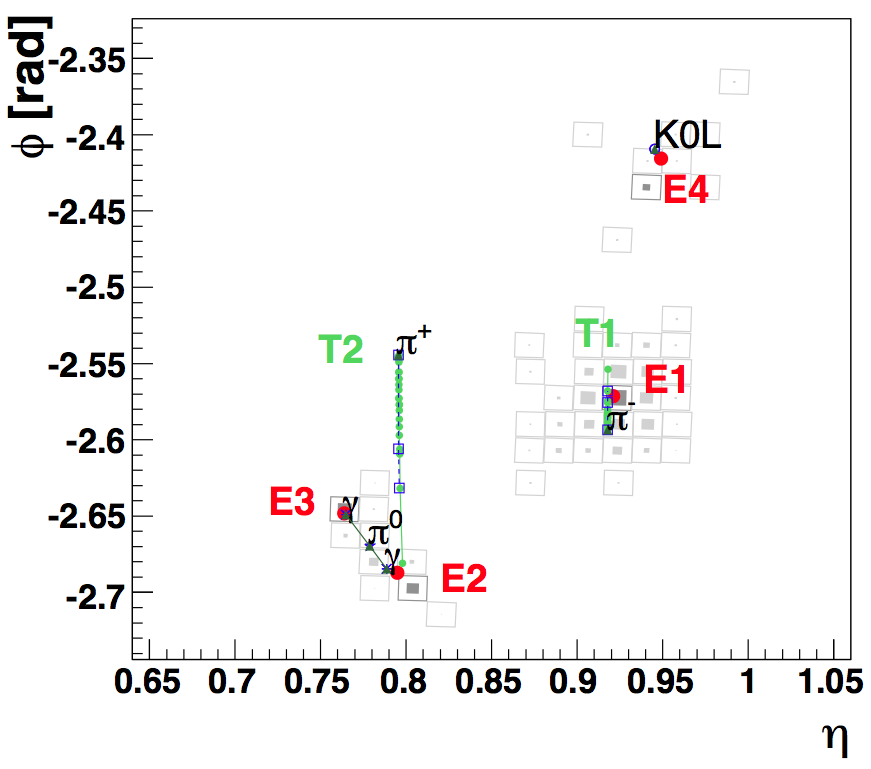
\includegraphics[width=\textwidth]{tex/reco/fig/reco-pf-2.png}
    \caption{ECAL energy in the $\eta-\phi$ plane}
    \label{fig:pf-2}
  \end{subfigure}
  \begin{subfigure}[b]{0.44\textwidth}
    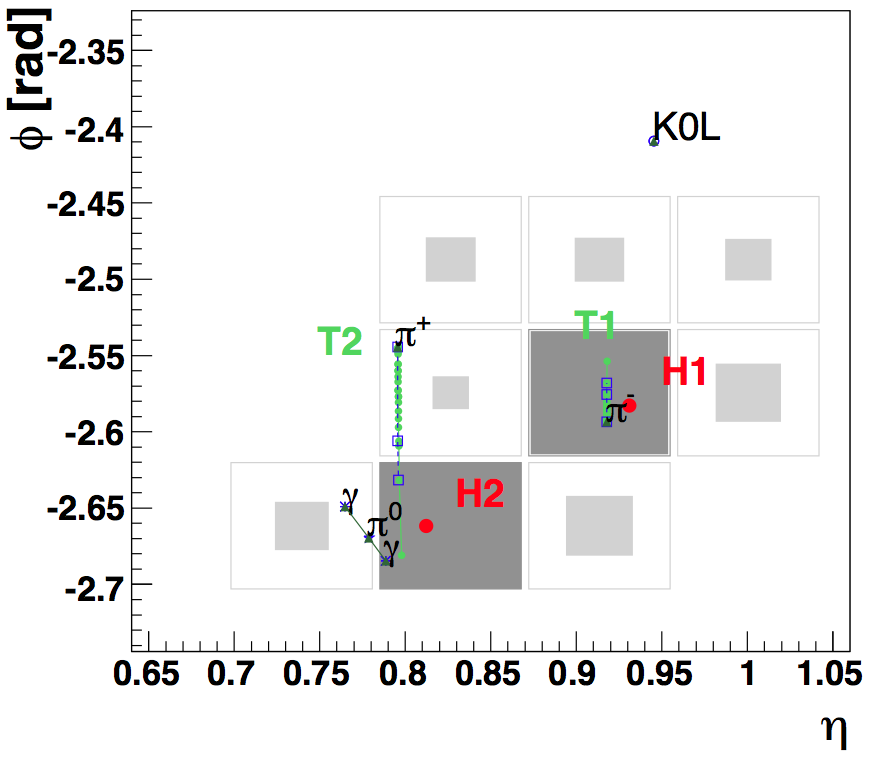
\includegraphics[width=\textwidth]{tex/reco/fig/reco-pf-3.png}
    \caption{HCAL energy in the $\eta-\phi$ plane}
    \label{fig:pf-3}
  \end{subfigure}
  \caption{
    An event display of a simulated simple hadronic jet with four 
    constituent particles ($\pi^+$, $\pi^-$, $\pi^0$, $\text{K}_{\text{L}}^0$)
    and a \pt~of 65 GeV interacting with the CMS inner tracker, ECAL, and HCAL.
    In all figures, 
    the reconstructed charged tracks from the $\pi^+$ and $\pi^-$ are shown as solid green lines, 
    the calorimetric energy cluster positions are shown as closed red markers,
    the simulated paths of the particles are shown dashed blue lines, and 
    the simulated positions of the particles' impacts with the calorimeters are shown as various open markers.  
    Figure (a) is shown in the $r-\phi$ plane.  The ECAL and HCAL surfaces are
    represented as black circles centered around the interaction point.
    Figure (b) is a view of the energy deposits in the ECAL as shown in the 
    $\eta-\phi$ plane.  The $\text{K}_{\text{L}}^0$,
    $\pi^-$, and photons from the $\pi^0 \rightarrow \gamma\gamma$ decay leave
    four well-separated clusters in the ECAL.  The $\pi^+$ leaves no energy
    in the ECAL.
    Figure (c) is a view of the two energy deposits in the HCAL as shown in the
    $\eta-\phi$ plane
    \cite{pf-1}.
  }
  \label{fig:pf}
\end{figure}


\subsection{Fundamental elements}

Two kinds of fundamental elements are important to this
discussion: charged particle tracks from the inner tracker
and calorimetric energy clusters from the ECAL and HCAL.

The reconstruction of charged particle tracks using data from
the inner tracker has been discussed in Section \ref{sec:reco-track}.
While the momentum of charged hadrons (e.g. pions) is measured
both by reconstructing tracks in the inner tracker and
by measuring the energy absorbed by the calorimeters, the 
resolution of the inner tracker's measurement is vastly superior
for charged hadrons with \pt~up to several hundreds of GeV.
This is important, because an average of roughly two thirds of a
jet's energy is carried by charged particles.
In addition, the tracker provides a precise measurement of the
trajectory of charged particles.  These two features make
charged particle tracks from the inner tracker a cornerstone of
the PF reconstruction algorithm.  In the simulated simple hadronic jet 
example of Figure \ref{fig:pf}, reconstructed tracks are represented
by solid green lines.

Calorimetric energy clusters are reconstructed using an algorithm specific to PF.
This algorithm has been 
developed with at least four goals in mind:
to detect and measure the energy and direction of 
stable neutral particles (like photons and neutral hadrons);
to separate these neutral particles from energy deposits originating from charged
hadrons;
to reconstruct and identify electrons and the photons associated with 
Bremsstrahlung radiation; and to ameliorate the energy measurement
of charged hadrons for which the track parameters were not determined
accurately (as is the case for low-quality or high-\pt~tracks).
The algorithm is performed separately in the EB, EE, PS, 
HB, and HE.  It is not performed in the HF, so each cell in the HF 
yields at most one cluster.  The algorithm consists 
of three steps.  First, the algorithm identifies seeds for the clusters
using local calorimeter cell energy maxima above a given energy.
Second, ``topological clusters'' are formed from these seeds by combining cells with 
at least one side in common with a cell already included in the cluster
and with an energy above a noise threshold (80 MeV in the EB, 300 MeV in the EE, and 800 MeV in the HCAL).
Finally, ``PF clusters'' are formed using topological clusters as seeds.
The number of PF clusters identified by the algorithm is equal 
to the number of cluster seeds identified.
In the simulated simple hadronic jet example of Figure \ref{fig:pf}, calorimetric energy clusters
in the ECAL and HCAL are represented by closed red markers \cite{pf-1}.

\subsection{Link algorithm}

In general, a particle passing through the CMS detector
is expected to give rise to more than one PF element.
For example, an electron may give rise to a charged particle
track and an ECAL energy cluster.  These various elements
are connected to each other using a linking algorithm in
order to reconstruct the original single particle.  The linking algorithm
is tentatively performed between each pair of elements, and the 
quality of the link is quantified using a distance (defined below).  The algorithm
then produces a ``block'' of linked elements.  Each block typically
contains 1-3 elements.  Three kinds of links are considered: 
between track and calorimeter cluster, between calorimeter cluster
and calorimeter cluster, and between track and track.

In the case of linking between a charged particle track and a calorimeter cluster,
the track is first extrapolated from its last measured hit in the tracker 
to all of the calorimeters to which the track is pointing.  These calorimeters include 
the PS for forward tracks, the EB and EE (corresponding to an electron shower), and the
HCAL (corresponding to a hadronic shower).  The original track is linked
to any cluster with boundaries that include the extrapolated track's position, but the 
cluster's boundaries may be expanded to account for the presence of gaps between cells,
dead cells, or uncertainty on the shower position.  The distance associated with the
link is defined as the distance in the $\eta$-$\phi$ plane between the 
position of the extrapolated track and the position of the cluster.

An additional case of track-to-cluster linking is defined to deal
with electrons undergoing Bremsstrahlung radiation.  In an attempt
to collect all of the energy carried away by Bremsstrahlung photons
emitted by electrons in the tracker, the tangents to tracks are extrapolated
to the ECAL from the intersection points of the track with an inner 
tracker layer.  A link is created if the extrapolated tangent is within
the boundaries of an ECAL cluster, as described in the previous paragraph.

Links may also be created between two calorimeter energy clusters: between
an ECAL cluster and an HCAL cluster, or between an ES cluster and an EE
cluster, for example.  Such a link is created when the cluster in the more 
granular detector lays within the $\eta-\phi$ envelope of the cluster in the
less granular detector.  As in the case of the track-to-cluster linking,
the envelopes may be slightly enlarged to reflect gaps between cells, dead cells,
and positional uncertainties. The distance associated with the link
is defined as the distance in the $\eta-\phi$ plane between the two cluster
positions.

Finally, a link may be created between a track from the inner tracker
and a track in the muon system.  Such a link is created for every
global muon for which the $\chi^2$ is below a defined maximum.  
If more than one global muon can be created from several tracker 
tracks and a given muon track, the algorithm keeps only the global 
muon with the lowest $\chi^2$.  The $\chi^2$ value defines the distance \cite{pf-1}.

\subsection{Particle reconstruction and identification}

Once links and blocks have been created by the PF linking 
algorithm, the PF reconstruction algorithm reconstructs 
particles from those blocks and identifies them.  After the reconstruction
algorithm has reconstructed a particle candidate, the corresponding 
block and its constituent elements are removed from consideration while constructing
additional particle candidates.
This results in a global event description, which can be used to 
reconstruct jets and to provide a \met~measurement.

Muons and electrons are first particles to be identified and reconstructed.
A global muon is identified as a ``PF muon'' if its 
momentum as measured by the combined fit is within three standard deviations
of the momentum measured by the tracker only.  Electrons are identified from blocks
containing a track and an ECAL energy cluster.  Electrons are pre-identified 
by using the tracker as a pre-shower: electrons are expected to have shorter
tracks and to lose energy as they proceed radially outward through the tracker.
These pre-identified electron tracks are fit with a GSF (see Section \ref{sec:reco-electron})
in order to determine their
trajectories.  Final identification of ``PF electrons'' depends on a number of pre-defined ECAL 
and inner tracker variables.

``PF charged hadrons'' are identified and reconstructed using tightly-selected
tracks from the inner tracker and calibrated energy clusters from the ECAL and HCAL.
The energy clusters are calibrated using Equation \ref{eqn:pf-calib}:
\begin{equation}
  E_{\text{calib}} = a + b(E,\eta)\cdot E_{\text{ECAL}} + c(E,\eta)\cdot E_{\text{HCAL}}
  \label{eqn:pf-calib}
\end{equation}
where $a$, $b(E,\eta)$, and $c(E,\eta)$ are coefficients whose values
were determined using a simulated sample of simulated single hadrons, $\eta$ is the 
pseudorapidity of the HCAL cluster,
$E_{\text{ECAL}}$ is the uncalibrated energy of the ECAL cluster,
$E_{\text{HCAL}}$ is the uncalibrated energy of the HCAL cluster, and 
$E$ is an estimate of the true energy of the hadron (either the total charged particle momentum, or the 
total uncalibrated calorimeter energy, whichever is larger).
Links between the selected tracks
and the HCAL clusters are then considered.  If an HCAL cluster is linked to
several tracks, then the sum of the track momenta is compared to the HCAL cluster.
If a single track is linked to several HCAL clusters, only the closest cluster
is kept for comparison.  Any ECAL clusters associated with the tracks under consideration
are ordered according to their distance to the closest track.  The list of ECAL clusters is 
scanned, and the cluster is kept so long as $E_{\text{calib}}$ is less than the total charged
particle momentum.

If, in the end, $E_{\text{calib}}$ is less than the sum of the momenta of the associated tracks,
the link is kept, and each remaining track in the block is reconstructed as a charged hadron,
the momentum and energy of which are taken from the track momentum under a charged pion 
mass hypothesis.  If $E_{\text{calib}}$ is significantly larger than the charged particle momentum 
(i.e. outside of the calorimeter energy resolution), then a ``PF photon'' or a 
``PF neutral hadron'' may be created with the energy associated with the excess.
If the excess is larger than the total $E_{\text{ECAL}}$, then a photon is created with the 
excess ECAL energy, and a neutral hadron is created with the excess HCAL energy.
Otherwise, only a photon is created.  The preference for photons is justified by the observation
that 25\% of jet energy is carried by photons, while neutral hadrons leave only 3\% of jet
energy in the ECAL.
Remaining ECAL and HCAL clusters which are not linked to tracks
give rise to PF photons and PF neutral hadrons.

The final list of reconstructed PF electrons, muons, taus (not discussed here),
charged hadrons, neutral hadrons, and photons are referred to collectively as 
``PF candidates'' \cite{pf-1}.
